\documentclass[fontsize=12pt]{article}
\usepackage[english,ngerman]{babel}
\usepackage[T1]{fontenc}
\usepackage[utf8]{inputenc}
\usepackage{amsmath,amssymb}
\usepackage[colorlinks=true,linkcolor=black,anchorcolor=black,citecolor=black,filecolor=black,menucolor=black,runcolor=black,urlcolor=black]{hyperref}
\usepackage{graphicx}
\usepackage{fancyhdr}
\usepackage{lastpage}
\usepackage{pgfplots}
\usepackage{datetime2}
\usepackage{tikz}
\usepackage{pdfpages}
\usetikzlibrary{arrows.meta,patterns}
\usepackage{acronym}
\usepackage{apacite}
\usetikzlibrary{ipe} % ipe compatibility library

\usepackage{geometry}
 \geometry{
 a4paper,
 left=35mm,
 right=25mm,
 top=20mm,
 bottom=20mm
 }

\renewcommand{\baselinestretch}{1.5}

\graphicspath{{./pictures/}}
\setlength\parindent{0pt}

\tikzstyle{ipe stylesheet} = [
  ipe import,
  even odd rule,
  line join=round,
  line cap=butt,
  ipe pen normal/.style={line width=0.4},
  ipe pen heavier/.style={line width=0.8},
  ipe pen fat/.style={line width=1.2},
  ipe pen ultrafat/.style={line width=2},
  ipe pen normal,
  ipe mark normal/.style={ipe mark scale=3},
  ipe mark large/.style={ipe mark scale=5},
  ipe mark small/.style={ipe mark scale=2},
  ipe mark tiny/.style={ipe mark scale=1.1},
  ipe mark normal,
  /pgf/arrow keys/.cd,
  ipe arrow normal/.style={scale=7},
  ipe arrow large/.style={scale=10},
  ipe arrow small/.style={scale=5},
  ipe arrow tiny/.style={scale=3},
  ipe arrow normal,
  /tikz/.cd,
  ipe arrows, % update arrows
  <->/.tip = ipe normal,
  ipe dash normal/.style={dash pattern=},
  ipe dash dotted/.style={dash pattern=on 1bp off 3bp},
  ipe dash dashed/.style={dash pattern=on 4bp off 4bp},
  ipe dash dash dotted/.style={dash pattern=on 4bp off 2bp on 1bp off 2bp},
  ipe dash dash dot dotted/.style={dash pattern=on 4bp off 2bp on 1bp off 2bp on 1bp off 2bp},
  ipe dash normal,
  ipe node/.append style={font=\normalsize},
  ipe stretch normal/.style={ipe node stretch=1},
  ipe stretch normal,
  ipe opacity 10/.style={opacity=0.1},
  ipe opacity 30/.style={opacity=0.3},
  ipe opacity 50/.style={opacity=0.5},
  ipe opacity 75/.style={opacity=0.75},
  ipe opacity opaque/.style={opacity=1},
  ipe opacity opaque,
]

\definecolor{red}{rgb}{1,0,0}
\definecolor{blue}{rgb}{0,0,1}
\definecolor{green}{rgb}{0,1,0}
\definecolor{yellow}{rgb}{1,1,0}
\definecolor{orange}{rgb}{1,0.647,0}
\definecolor{gold}{rgb}{1,0.843,0}
\definecolor{purple}{rgb}{0.627,0.125,0.941}
\definecolor{gray}{rgb}{0.745,0.745,0.745}
\definecolor{brown}{rgb}{0.647,0.165,0.165}
\definecolor{navy}{rgb}{0,0,0.502}
\definecolor{pink}{rgb}{1,0.753,0.796}
\definecolor{seagreen}{rgb}{0.18,0.545,0.341}
\definecolor{turquoise}{rgb}{0.251,0.878,0.816}
\definecolor{violet}{rgb}{0.933,0.51,0.933}
\definecolor{darkblue}{rgb}{0,0,0.545}
\definecolor{darkcyan}{rgb}{0,0.545,0.545}
\definecolor{darkgray}{rgb}{0.663,0.663,0.663}
\definecolor{darkgreen}{rgb}{0,0.392,0}
\definecolor{darkmagenta}{rgb}{0.545,0,0.545}
\definecolor{darkorange}{rgb}{1,0.549,0}
\definecolor{darkred}{rgb}{0.545,0,0}
\definecolor{lightblue}{rgb}{0.678,0.847,0.902}
\definecolor{lightcyan}{rgb}{0.878,1,1}
\definecolor{lightgray}{rgb}{0.827,0.827,0.827}
\definecolor{lightgreen}{rgb}{0.565,0.933,0.565}
\definecolor{lightyellow}{rgb}{1,1,0.878}
\definecolor{black}{rgb}{0,0,0}
\definecolor{white}{rgb}{1,1,1}

\pagestyle{fancy}
\fancyhf{}
\lfoot{B. Blacher, F. Weissenbacher}
\lhead{Modellauto mit Sensorik}
\rhead{
\includegraphics[scale=0.5]{htllogo.png}}
\rfoot{\thepage{}}
 
\begin{document}
\begin{titlepage}
	\centering
	\hspace{1.5cm}
	
\includegraphics[scale=2]{htllogo.png}
	\newline
	{\huge Diplomarbeit \par}
	{\Large Fachbereich Mechatronik\par}
	\vspace{1.5cm}
	{\huge Modellauto mit Sensorik\par}
	\vspace{2cm}
	{\Large verfasst und vorgelegt von\par}
	{\huge Benjamin Blacher\par}
	{\huge Florian Weissenbacher\par}
	\vfill
	betreut von\par
	Dipl. Ing. Wolfgang \textsc{Czernin}\par
	Dipl. Ing. Matthias \textsc{Dirl}

	\vfill

% Bottom of the page
	{\large Kapfenberg, \today\par}
\end{titlepage}
\newpage

%Tikz example
%\begin{figure}[h]
%\centering
%\begin{tikzpicture}[ipe stylesheet]
%%content
%\end{tikzpicture}
%\caption{Sender-Empfänger-Modell}
%\label{fig:SenderEmpfaenger}
%\end{figure}

%section example
%\section{xxx}
%\label{sec:xxx}

%subsection example
%\subsection{xxx}}
%\label{subsec:xxx}

%image example
%\begin{figure}[h]
%\centering
%\includegraphics[scale=0.1]{*.*}
%\caption{xxx}
%\label{fig:xxx}
%\end{figure}
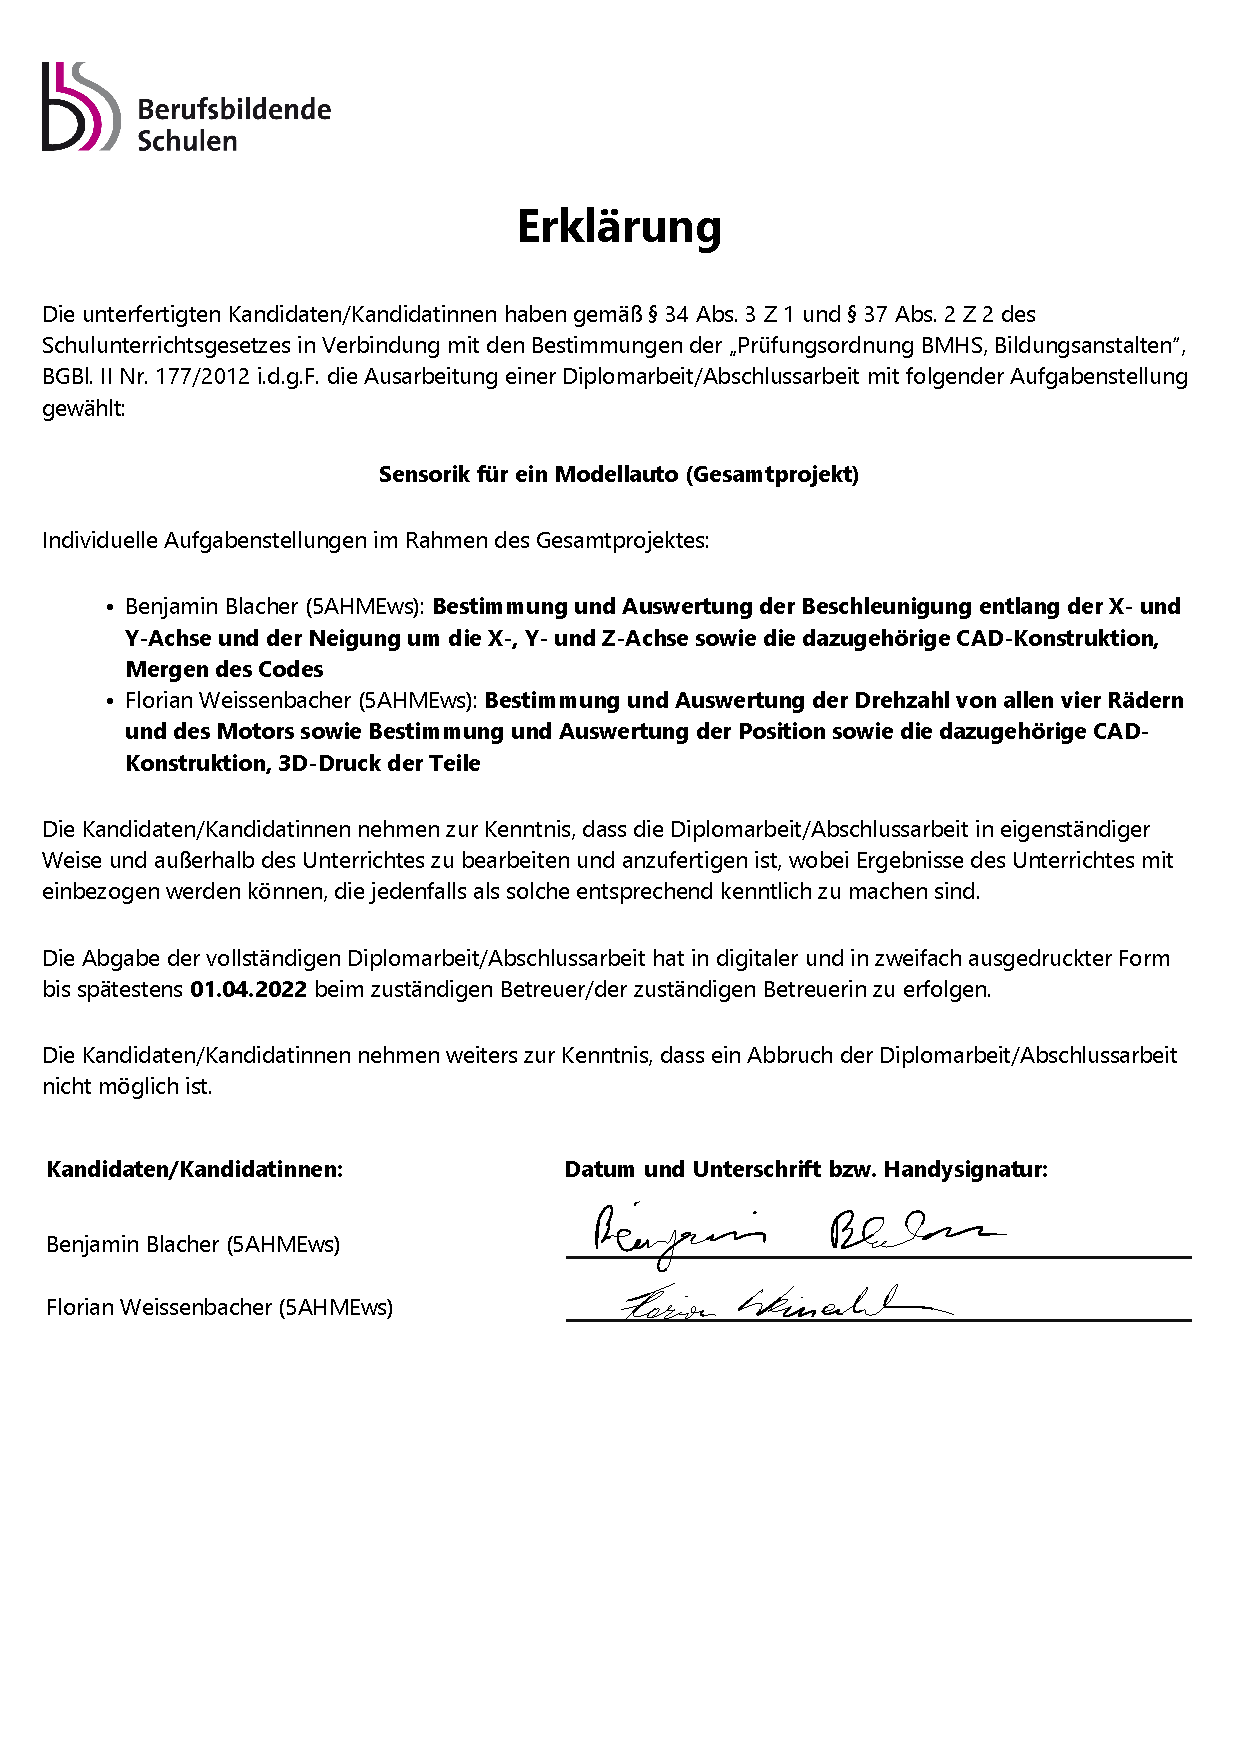
\includegraphics[page=1, scale=0.7]{./sources/DADB.pdf}
\newpage
\section2{Eidesstattliche Erklärung}
\label{sec:eidesstattlErkl}
Ich erkläre eidesstattlich, dass ich die Arbeit selbständig angefertigt, keine anderen als die an-gegebenen Hilfsmittel benutzt und alle aus ungedruckten Quellen, gedruckter Literatur oder aus dem Internet im Wortlaut oder im wesentlichen Inhalt übernommenen Formulierungen und Konzepte gemäß den Richtlinien wissenschaftlicher Arbeiten zitiert, durch Fußnoten gekenn-zeichnet bzw. mit genauer Quellenangabe kenntlich gemacht habe.

\vspace{2cm}
\hspace{2cm}\hrulefill{}\hspace{2.35cm}\hrulefill{}\hspace{1cm}

\hspace{2cm} Ort, Datum \hspace{5cm} Benjamin Blacher \hfill

\vspace{2cm}
\hspace{2cm}\hrulefill{}\hspace{2.35cm}\hrulefill{}\hspace{1cm}

\hspace{2cm} Ort, Datum \hspace{5cm} Florian Weissenbacher \hfill
\newpage
\begin{otherlanguage}{english} 
\begin{abstract}
\noindent
Various forces and moments act on cars while driving. Although these variables are measured in real cars, they are not made directly accessible to the driver. Instead, they are used for various systems such as ABS or traction control. In order to make these parameters evaluable, a remote-controlled model car is to be equipped with sensor technology. Factors relevant to driving dynamics include accelerations as well as the orientation in three-dimensional space and the speeds of the four wheels. Furthermore, the location of the vehicle is to be recorded with the help of the \ac{GPS}. Separate housings and mountings are to be made for the installation of the electronics. A single-board computer from the Raspberry Pi Foundation is being used to enable the storage of data on the remote-controlled car. It is also important that the collected data can be analysed and displayed with a user-friendly graphical interface. \\
This diploma thesis was carried out in the course of the standardised diploma examination at the HTL Kapfenberg as well as financed by the HTL. In the future, this diploma thesis will be used for educational purposes.
\end{abstract}
\end{otherlanguage}
\newpage
\begin{abstract}
\noindent
Auf Autos wirken während der Fahrt diverse Kräfte und Momente. Diese Größen werden bei realen Autos zwar gemessen, für den Fahrer aber nicht direkt zugänglich gemacht. Stattdessen werden sie für verschiedene Systeme wie ABS oder Traktionskontrolle verwendet. Um diese Kenngrößen auswertbar zu machen, soll ein ferngesteuertes Modellauto mit Sensorik ausgestattet werden. Für die Fahrdynamik relevante Faktoren sind unter anderem die Beschleunigungen sowie die Lage im dreidimensionalen Raum und die Drehzahlen der vier Räder. Weiters ist der Standort des Fahrzeuges mithilfe des \ac{GPS} aufzuzeichnen. Für die Unterbringung und Montage der Elektronik sind eigene Gehäuse sowie Befestigungen anzufertigen. Um die korrekte Speicherung der Daten am ferngesteuerten Auto zu ermöglichen wird ein Einplatinencomputer der Raspberry Pi Foundation verwendet. Außerdem ist es wichtig, dass die erfassten Daten mit einer benutzerfreundlichen grafischen Oberfläche ausgewertet und dargestellt werden können. \\
Diese Diplomarbeit wurde im Zuge der standardisierten Reife- und Diplomprüfung an der HTL Kapfenberg durchgeführt sowie von dieser finanziert. In Zukunft soll diese Arbeit für Lehrzwecke verwendet werden.
\end{abstract}
\newpage
\tableofcontents
\newpage
\section{Einleitung}
\label{sec:einleitung}
Diese Diplomarbeit handelt von der Ausstattung eines ferngesteuerten Autos mit Sensorik, finanziert wurde sie von der HTL Kapfenberg.\\
Das Ziel ist es, verschiedene Kenngrößen, die eine Analyse des Fahrverhaltens ermöglichen, zu messen. Darunter fallen die Beschleunigung entlang der x- und y-Achse, die Neigung um die x-, y- und z-Achse, die Drehzahl von allen vier Rädern sowie die Position. Diese Daten sind digital festzuhalten und anschließend auszuwerten. \\
Um dies zu erreichen werden passende Sensoren sowie ein Einplatinencomputer zur Datenverarbeitung ausgewählt. Zur Befestigung der gewählten Elektronik werden Halterungen mithilfe von \ac{CAD}-Software konstruiert und anschließend mit verschiedenen 3D-Druck-Verfahren gefertigt. Die Spannungsversorgung der Bauteile erfolgt über die vom RC-Auto verwendeten Akkus, wessen Spannung auf die notwendige herabgewandelt wird. Außerdem werden die Sensoren in einem gemeinsamen Python-Programm eingebunden um die Sammlung der Daten in einer einzelnen Datei (als .txt - mit Kommas getrennt) zu ermöglichen. Weiters kann mittels Knopfdruck zwischen zwei Modi gewechselt werden, welche mit dem Status einer \ac{LED} unterschieden werden können. Zum Einen steht das Aufzeichnen der Daten zur Verfügung, andererseits können die gesammelten Daten auf einen \ac{USB} Datenträger übertragen werden. \\
Die Auswertung der Daten wird mithilfe einer eigens geschriebenen Desktop-Anwendung vereinfacht, diese wird ebenfalls mithilfe von Python umgesetzt. Zusätzlich wird das Grafikoberflächen-toolkit Qt für das Darstellen der Fenster verwendet.
\newpage
\section{Theoretische Grundlagen}
\label{sec:theoretGrundl}
Dieses Kapitel behandelt die theoretischen Grundlagen für verwendete Verfahren, Hardware und Software. Es hat die Aufgabe den Leser:innen für das Verständnis essentielle Informationen zu übermitteln.
\subsection{Globales Positionsbestimmungssystem}
\label{subsec:tGPS}
Das \ac{GPS} ist ein gängiges Navigationssystem, um die geografische Position zu ermitteln. Ursprünglich wurde \ac{GPS} für militärische Zwecke entwickelt und wird heutzutage vom Verteidigungsministerium der USA betrieben.\\
\ac{GPS} ist satellitengestützt und umfasst eine Anzahl von 32 Satelliten in der Erdumlaufbahn, wovon mindestens vier eine Verbindung mit dem GPS-Empfängermodul haben müssen, um die Position bestimmen zu können. Drei dieser Satelliten sind für die Erfassung der Längen- und Breitengrade, sowie die der Höhe notwendig, die Verbindung mit einem vierten Satelliten ermöglicht die Synchronisation der Uhr des Empfängers, mit der der Satelliten. Dies ist besonders ausschlaggebend, da nur bei einer exakten Übereinstimmung der Zeiten, die Position korrekt berechnet werden kann. Um die Position zu berechnen, wird die Zeit gemessen, die das Signal vom Satelliten zum Empfänger benötigt und in eine Distanz umgerechnet. Mithilfe der Entfernungen zu mehreren Satelliten vom Empfänger, kann über Triangulation die geografische Lage auf der Erdoberfläche ermittelt werden.\\
Die Genauigkeit der Positionserfassung variiert zwischen 13 Meter und 1 Millimeter. Abweichungen unter einem Meter sind allerdings fast nur mit professioneller, beziehungsweise militärischer Ausrüstung erreichbar. Mit Komponenten aus den Hobby-Elektronikbereich sowie in Smartphones, sind Genauigkeiten zwischen 13 und 3 Metern realistisch möglich.\\
Die Daten werden standardisiert im \ac{NMEA}-Format über eine serielle Schnittstelle ausgegeben. (\cite{schnabelGPS})


\subsection{Inertiale Messeinheit}
\label{subsec:tIMU}
Eine \ac{IMU} z. Dt. inertiale Messeinheit kombiniert mehrere verschiedene Sensoren zur Bestimmung von Lage, Beschleunigungen und Position im dreidimensionalen Raum. Um eine zuverlässige Ermittlung dieser Werte zu gewährleisten, werden Beschleunigungsmessung, Rotationsgeschwindigkeitsmessung (und in einigen Fällen auch die Messung des Magnetfeldes der Erde) kombiniert. Inertiale Messeinheiten werden unter anderem für die Navigation von Flugzeugen, Raumschiffen und Schiffen verwendet. In der Automobilindustrie werden \ac{IMU}s verwendet, um das Fahrverhalten von Autos zu bestimmen und dieses zu verbessern.\\
Die \ac{IMU} liefert die Beschleunigungen sowohl in x-, y- als auch z-Richtung, die Winkelgeschwindigkeiten um die x-, y- als auch z-Achse (und in manchen Fällen die magnetische Feldstärke in x-, y- als auch z-Richtung). Um die Lage zu bestimmen können die Beschleunigungssensoren verwendet werden, indem die Lage der Erdbeschleunigung im dreidimensionalen Raum ermittelt wird, dies funktioniert allerdings nur, solange der Sensor sich in Ruhelage befindet. Alternativ können die Rotationsgeschwindigkeiten integriert werden, dies ergibt aber aufgrund von Messfehlern nach einiger Zeit Abweichungen (drift).\\ Um eine fehlerfreie Ermittlung der Lage zu ermöglichen kann Sensorfusion betrieben werden. Darunter versteht man einen Prozess, der Signale von zwei oder mehr Sensoren zusammenfasst. Im Falle einer \ac{IMU} kann die Ermittlung mittels Accelerometern, Gyroskopen und Magnetometern wie in Sektion \ref{subsec:IMUprogram} beschrieben kombiniert werden.
(\cite{UCAM-CL-TR-696})
\begin{figure}[h]
\centering
\missingfigure{}
\caption{Eine \ac{IMU} in einem \ac{3D}-Koordinatensystem}
\label{fig:IMU3D}
\end{figure}

\subsection{Hall-Effekt-Sensor}
\label{subsec:tHall}

\subsection{Infrarot-Lichtschranke}
\label{subsec:tIR}

\subsection{Raspberry Pi Zero 2 W}
\label{subsec:tRasPi}
Der Raspberry Pi Zero 2 W ist ein Einplatinencomputer der Raspberry Pi Foundation. Mit einem 1 \ac{GHz} quad-core 64-bit Arm Prozessor, 512 \ac{MB} \ac{SDRAM}, eingebauten \ac{WLAN}- und Bluetooth-Modulen und 40 pins für \ac{GPIO}, \ac{SPI}, \ac{I2C}, \ac{UART} und Spannungsversorgung stellt er ein umfangreiches Paket für die Interaktion mit diverser Sensorik dar. Als Betriebssystem bietet die Raspberry Pi Foundation eine auf Debian basierte Linux-Distribution namens Raspberry Pi \ac{OS} an. Raspberry Pi \ac{OS} ist in drei verschiedenen Varianten verfügbar, diese unterscheiden sich im Funktionsumfang und der Installationsgröße. Aufgrund der limitierten Rechenleistung des \ac{Raspi} Zero 2 W und der fehlenden Notwendigkeit für eine Desktop-Umgebung ist die Lite-Version am besten geeignet.
\begin{figure}[h]
\centering
\missingfigure{}
\caption{Das Commandline-Tool neofetch am Raspberry Pi Zero 2 W}
\label{fig:pineofetch}
\end{figure}

\subsection{Python}
\label{subsec:tPython}
Python ist eine in den frühen 1990ern von Guido van Rossum erstellte Programmiersprache. Heutzutage zeichnet sich Python dadurch aus, dass es quelloffen und für jeden nutzbar ist. Außerdem nimmt Python dem Programmierenden durch die im Vergleich zu Sprachen wie C++ einfache Syntax und das integrierte Ressourcenmanagement viel Arbeit ab. Ein Nachteil von Python ist, dass es im Vergleich mit anderen Sprache wie C++ eine sehr langsame Programmiersprache ist. Aufgrund seiner Simplizität und Verfügbarkeit für Plattformen wie Microsoft Windows, macOS, Linux und FreeBSD gibt es sehr viele quelloffene Bibliotheken für Python, was das Programmieren noch weiter erleichtert. Ein weiterer Unterschied zu Sprachen wie C, C++ oder Rust besteht darin, dass Python interpretiert statt kompiliert wird. Dies hat zur Folge, dass der Code direkt ausgeführt werden kann, solange ein geeigneter Python-Interpreter und die verwendeten Bibliotheken installiert sind, ohne zuvor für jede Plattform eigens kompiliert werden zu müssen.
(\cite{matthes-2019})

\subsection{Qt}
\label{subsec:tQt}
Qt ist eine von der Qt Company entwickelte Bibliothek für die Entwicklung von grafischen Oberflächen. Sie ist wie Python plattformübergreifend und unterstützt unter anderem Microsoft Windows, macOS, Unixartige Betriebssysteme mit X11, Linux mit Wayland, Android und iOS. Qt unterstützt ebenfalls die Entwicklung mit verschiedenen Programmiersprachen, darunter Python, C++ und Qt Modeling Language, zusätzlich wird Unterstützung für Rust und Go von der Qt-Community angeboten. Qt ist wie Python Quelloffen und kann für die Open-Source-Programmierung frei verwendet werden. Die neueste Qt-Python Bibliothek heißt PySide6, mit nur fünf Zeilen Python-Code kann ein leeres Fenster erstellt werden.
\begin{figure}[h]
\centering

\includegraphics[scale=0.5]{EmptyQtWindow.png}
\caption{Leeres PySide6-Fenster auf Linux unter X11}
\label{fig:EmptyQtWindow}
\end{figure}

\subsection{FDM-3D-Druck}
\label{subsec:tFDM}
\ac{FDM} z. Dt. Schmelzschichtung, ist eine gängige Methode der additiven Fertigung, die auch die Funktionsweise der meisten \ac{3D}-Drucker darstellt. Additive Fertigung bedeutet, dass ein zu herstellendes \ac{3D}-Modell in einzelnen Schichten mit der gewünschten Schichthöhe auf einer Plattform aufgetragen wird. Der Vorteil ist, die Möglichkeit komplexe Modelle zu fertigen, die mit herkömmlichen Fertigungsverfahren sehr schwer, oder gar unmöglich sind.\\
Bei der \ac{FDM}-Technologie wird ein Kunststoffdraht (Filament) durch eine erhitzte Düse gepresst, wodurch der Kunststoff geschmolzen und je nach Düsenöffnung, in einem bestimmten Durchmesser extrudiert wird. Bei der \ac{FDM}-Methode können also ausschließlich Thermoplaste als Druckmaterial verwendet werden. Die Düse wird während dem Extrudier-Vorgang in einer bestimmten Höhe über einer (meist beheizten) Plattform, dem sogenannten Druckbett, bewegt, um die erste Schicht des Modells aufzutragen. Anschließend wird die Düse eine Schichthöhe angehoben, um die nächste Schicht auf der ersten aufzutragen (Siehe Abbildung \ref{fig:FDM}). Typische Schichthöhen von \ac{FDM}-Druckern sind 0,1 bis 0,4 Millimeter und die Düse hat meist einen Durchmesser von 0,4 Millimeter. Zu den möglichen Materialien zählen unter anderem \ac{PLA}, \ac{ABS}, \ac{PETG} sowie Nylon. Auch flexible Materialien sind möglich, welche meist mit erhöhten Drucker-Anforderungen verbunden sind. Bei Hobby-Druckern beträgt die typische maximale Druckgröße zwischen 120*120*120 und 300*300*300 Millimeter in x-, y-, und z-Richtung. Der große Nachteil von \ac{FDM} ist die Oberflächenbeschaffenheit des fertigen Bauteils, welche markante Rillen der einzelnen Schichten aufweist. (\cite{alexandreFDM})
\begin{figure}[h]
\centering
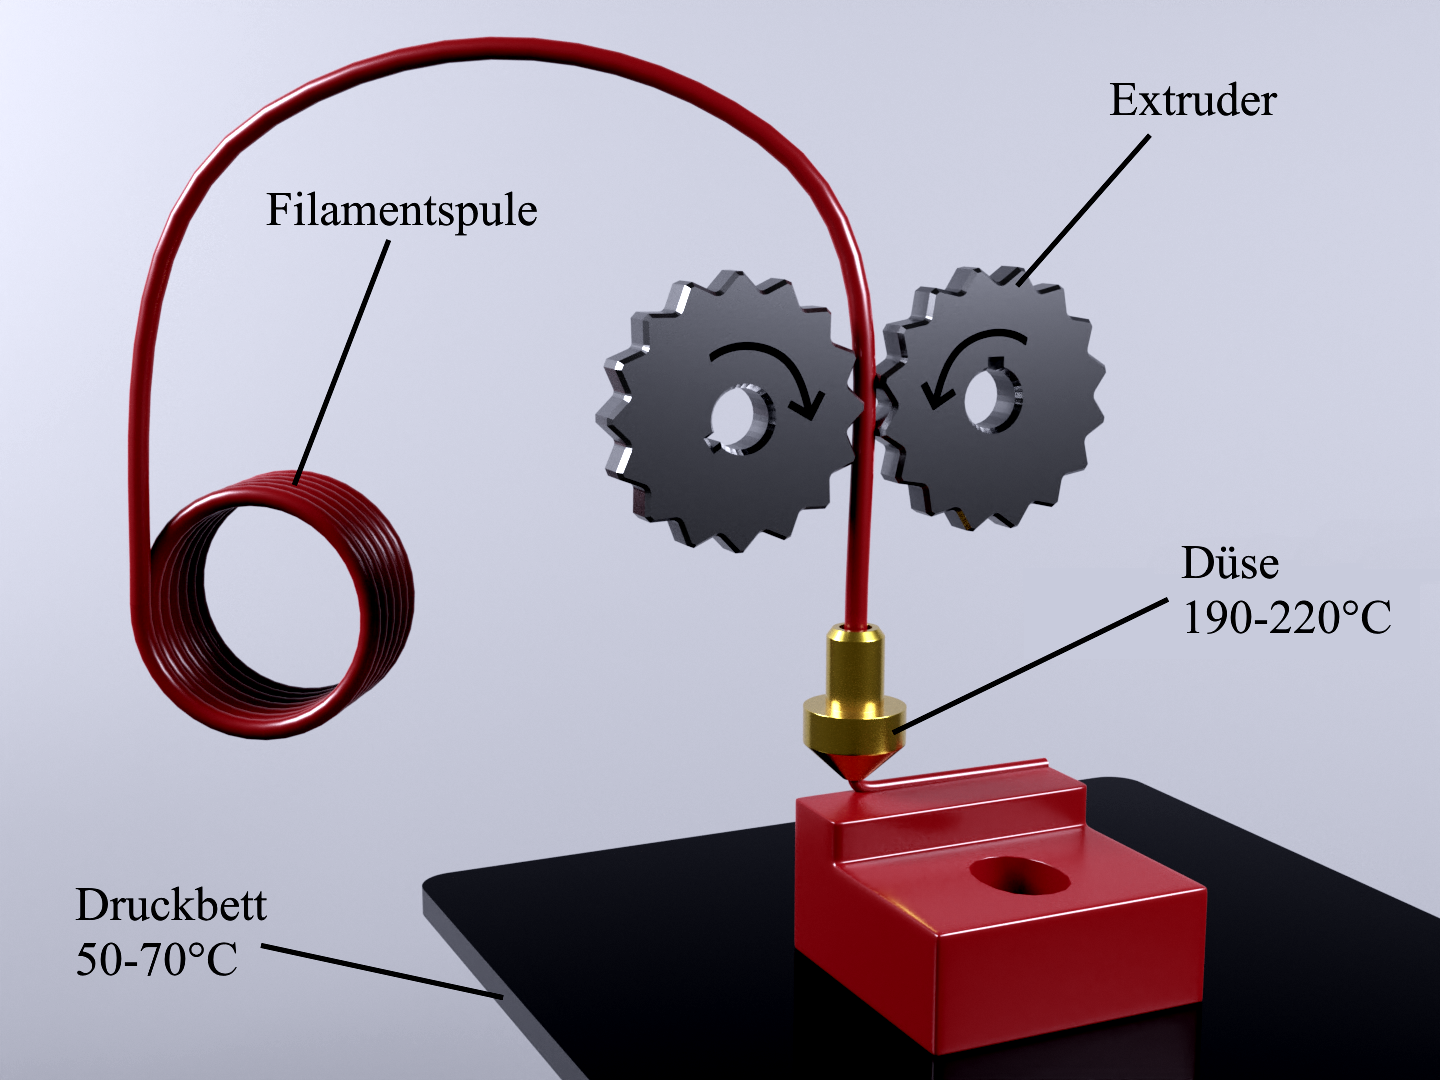
\includegraphics[scale=0.2]{FDM.png}
\caption{FDM-Funktionsweise}
\label{fig:FDM}
\end{figure}

\subsection{DUP-3D-Druck}
\label{subsec:tDUP}
\ac{DUP} ist eines der additiven Fertigungsverfahren, bei dem ein fotosensitives Harz Schicht für Schicht ausgehärtet wird, um ein \ac{3D}-Modell zu fertigen. Bei \ac{DUP} wird eine Plattform kopfüber in einen, mit einem speziellen Harz befüllten, Behälter gesenkt, bis diese eine Schichthöhe vom Boden des Behälters entfernt ist. Der Boden dieses Beckens besteht aus einem durchsichtigen Kunststoff und darunter befindet sich ein \ac{LCD}, welches, anders als herkömmlich, eine \ac{UV}-Leuchtdioden-Matrix als Hintergrundbeleuchtung aufweist. Das \ac{LCD} dient als Schablone und lässt nur dort \ac{UV}-Licht durchscheinen, wo das \ac{UV}-sensitive Harz ausgehärtet (polymerisiert) werden soll . Die erste ausgehärtete Harz-Schicht haftet an der Druckplattform, welche anschließend für die nächste eine Schichthöhe angehoben wird. Somit wird jeweils eine Schicht auf einmal gefertigt (Siehe Abbildung \ref{fig:DUP}).\\ Harz-Drucker sind bekannt dafür, dass sie eine deutlich bessere Druckqualität liefern können, als \ac{FDM}. Der Grund dafür sind zum einen die typischen Schichthöhen von 0.025 bis 0.1 Millimeter sowie die erhöhte Auflösung in x- und y-Richtung, welche abhängig von der \ac{LCD}-Auflösung ist.  Harz-Drucker haben also den großen Vorteil, dass (fast) keine Schicht-Rillen zu erkennen und viel detailliertere Modelle druckbar sind. Die maximale Druckgröße ist in den meisten Fällen kleiner als bei \ac{FDM}-Druckern und liegt im Durchschnitt bei etwa 180*120*200 Millimeter. Die Wellenlänge des \ac{UV}-Lichts der LEDs beträgt zwischen 395 und 405 Nanometer, was ebenfalls dem sensitiven Bereich des Harzes entsprechen muss. Nachdem ein Druck fertiggestellt wurde, ist dieses Modell immer noch mit flüssigem Harz überzogen, welches mit Alkohol entfernt werden muss. Da die Aushärtezeit beim Druckprozess pro Schicht nur circa zwei Sekunden dauert, muss das fertige Modell mit einer \ac{UV}-Lichtquelle erneut für 5 bis 10 Minuten ausgehärtet werden, um seine endgültigen Material-Eigenschaften zu erhalten. Mittlerweile gibt es einige Unternehmen, welche Harze mit besonderen Eigenschaften anbieten, wie zum Beispiel erhöhte Festigkeit, Zähigkeit oder mechanisch bearbeitbar.\\
\ac{DUP} und andere Harz-Druckverfahren haben also den großen Nachteil, dass sehr viel Aufwand im Bezug auf die Nachbearbeitung besteht und immer mit ausreichend Schutzkleidung, wie Handschuhe und Schutzbrille gearbeitet werden muss, da die Harze gesundheitsschädlich sein können. (\cite{druckwegeDUP})
\begin{figure}[h]
\centering
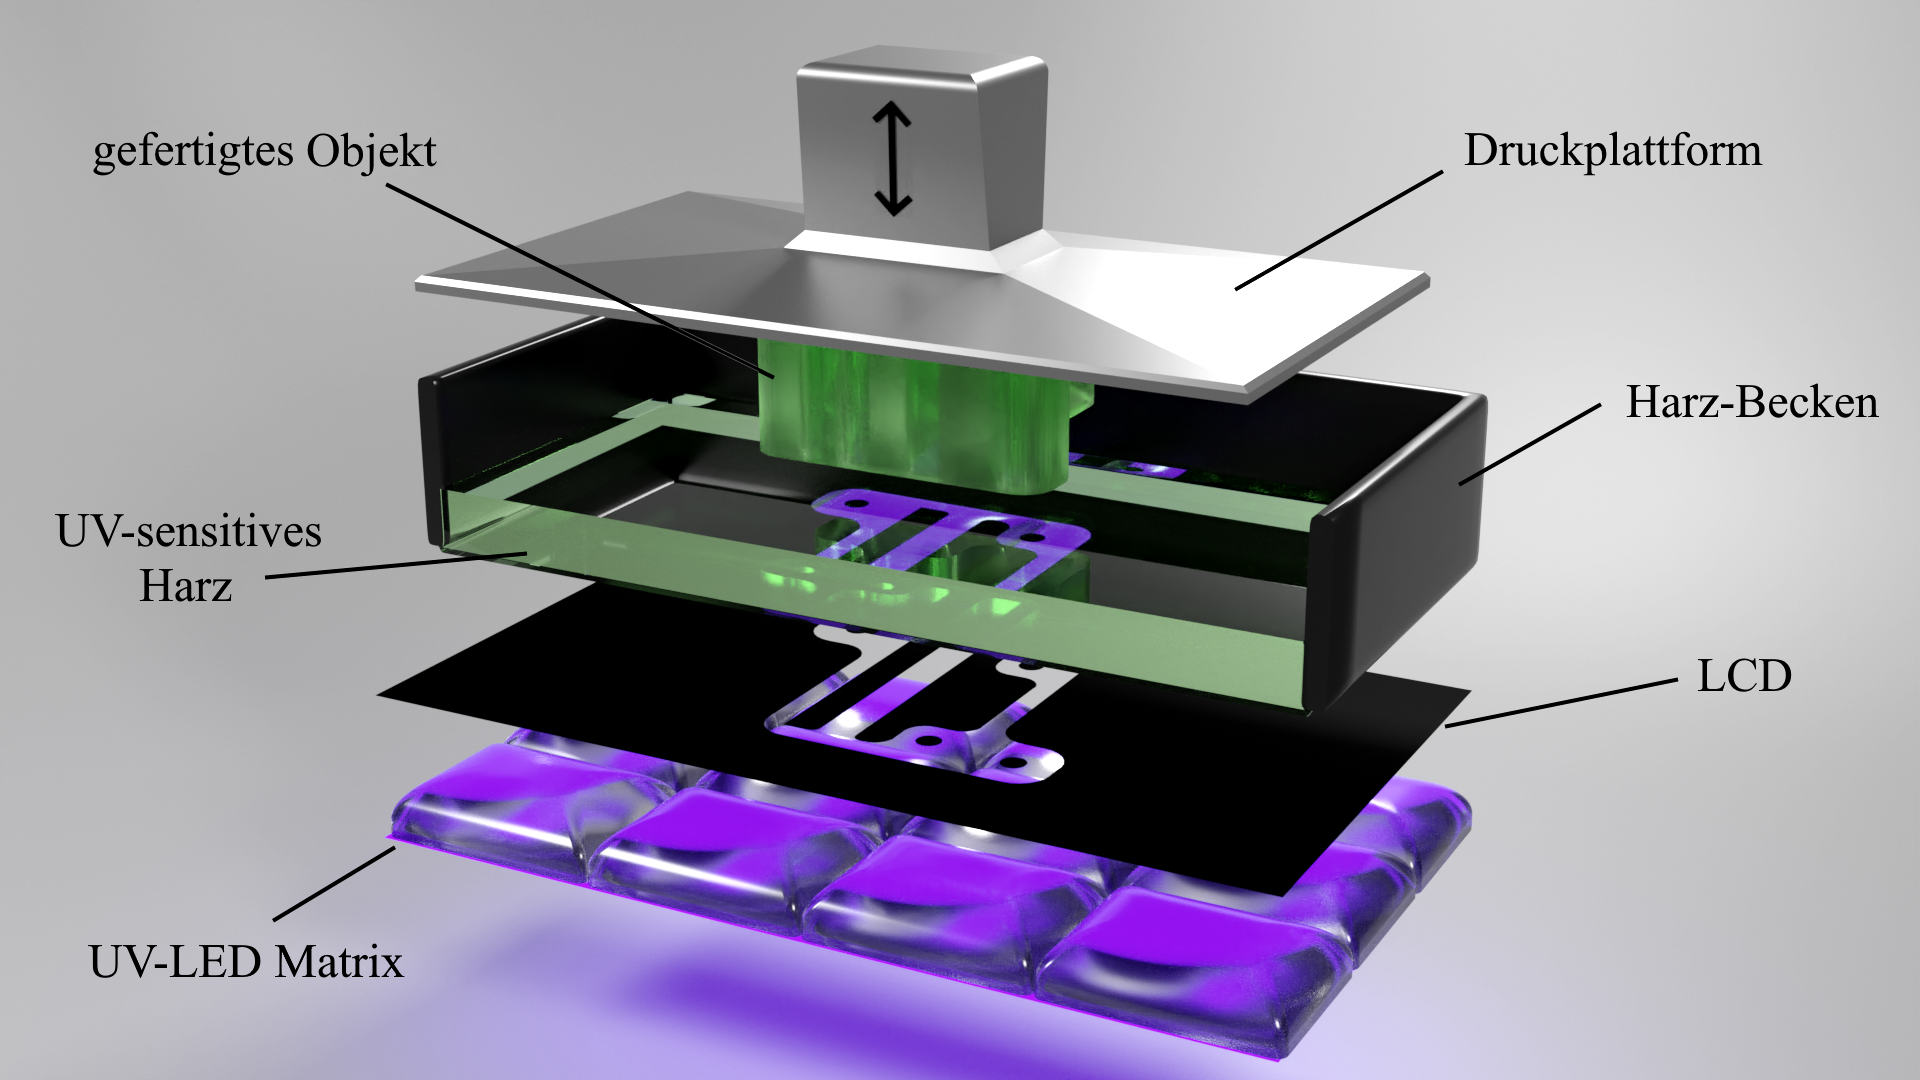
\includegraphics[scale=0.2]{DUP.png}
\caption{DUP-Funktionsweise}
\label{fig:DUP}
\end{figure}
\newpage
\section{Realisierungskonzepte}
\label{sec:realisierungskonzepte}
\newpage
\section{Technische Umsetzung}
\label{sec:technUmsetzung}
\newpage
\section{Zusammenfassung}
\label{sec:zusammenfassung}
\newpage
\bibliographystyle{apacite}
\bibliography{bibliography.bib}
\newpage
\listoffigures
\newpage
\listoftables
\newpage
\section{Abkürzungsverzeichnis}
\label{sec:Abkuerzungsverzeichnis}

\begin{acronym}
\acro{GPS}{Global Positioning System}
\end{acronym}

\begin{acronym}
\acro{IMU}{Inertial measurement unit}
\end{acronym}

\begin{acronym}
\acro{RPM}{Revolutions per minute}
\end{acronym}

\begin{acronym}
\acro{I2C}{Inter-Integrated Circuit}
\end{acronym}

\begin{acronym}
\acro{CAD}{Computer aided design}
\end{acronym}

\begin{acronym}
\acro{Raspi}{Raspberry Pi}
\end{acronym}

\begin{acronym}
\acro{USB}{Universal Serial Bus}
\end{acronym}

\begin{acronym}
\acro{NMEA}{National Marine Electronics Association}
\end{acronym}

\begin{acronym}
\acro{FDM}{Fused Deposition Modeling}
\end{acronym}

\begin{acronym}
\acro{PLA}{Polyactid}
\end{acronym}

\begin{acronym}
\acro{ABS}{Acrylnitril-Butadien-Styrol}
\end{acronym}

\begin{acronym}
\acro{PETG}{Polyethylenterephthalat-Glycol}
\end{acronym}


\end{document}